% J11: MILP design of PV + Li-ion + alkaline electrolyser for an energy-independent home (GIS, Italy)
% Shared preamble for the graphical abstracts (homepage "Latest journal articles").
% Build: bash _tikz/papers/build.sh  (writes images/papers/Jxx.svg)
% Classic TikZ look: white background, black text and arrows, standard xcolor
% colors for the elements (independent of the website theme).
\documentclass[tikz,border=0pt]{standalone}
\usepackage[T1]{fontenc}
\usepackage{textcomp}
\usepackage[scaled=0.95]{helvet}
\renewcommand\familydefault{\sfdefault}
\usetikzlibrary{arrows.meta,calc,positioning,patterns,decorations.pathreplacing}
% ---- classic colors (xcolor names) ----
\colorlet{main}{blue!70!black}   % primary elements
\colorlet{lite}{blue!35}         % connections
\colorlet{pale}{blue!8}          % light fills
\colorlet{acc}{red!75!black}     % highlights / outputs
\colorlet{good}{green!55!black}  % storage, positive
\colorlet{warn}{orange!85!black} % uncertain
\colorlet{sun}{orange}
\colorlet{rule}{black!35}
\colorlet{ink}{black}
\colorlet{muted}{black!60}
\colorlet{bg}{white}
\tikzset{
  every picture/.style={line cap=round, line join=round},
  head/.style={font=\fontsize{8.5}{10}\selectfont\bfseries, text=ink},
  sub/.style={font=\fontsize{6.6}{8}\selectfont, text=muted},
  lab/.style={font=\fontsize{7.2}{8.6}\selectfont, text=ink},
  flow/.style={-{Stealth[length=2.2mm,width=2mm]}, draw=black, line width=0.9pt},
  card/.style={draw=black!60, line width=0.6pt, fill=white, rounded corners=1mm},
  banner/.style={draw=black, line width=0.6pt, fill=black!4, text=black,
                 font=\fontsize{7.4}{9}\selectfont\bfseries\boldmath, inner sep=1.6mm},
}
% canvas 8 x 6 cm (4:3), white
\newcommand\canvas{\fill[bg] (0,0) rectangle (8,6);}

\begin{document}
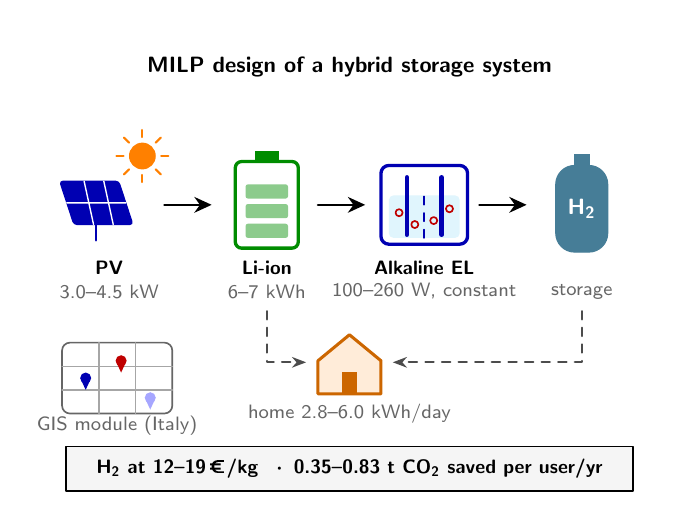
\begin{tikzpicture}
\canvas
\node[head] at (4,5.5) {MILP design of a hybrid storage system};
% ---- PV ----
\begin{scope}[shift={(0.95,3.75)}]
  \fill[sun] (0.42,0.62) circle (0.17);
  \foreach \a in {0,45,...,315} \draw[sun, line width=0.8pt] ($(0.42,0.62)+(\a:0.24)$) -- ($(0.42,0.62)+(\a:0.33)$);
  \filldraw[fill=main, draw=main, rounded corners=0.4mm] (-0.45,-0.25) -- (0.3,-0.25) -- (0.12,0.3) -- (-0.63,0.3) -- cycle;
  \draw[white, line width=0.5pt] (-0.54,0.025) -- (0.21,0.025) (-0.2,-0.25) -- (-0.32,0.3) (0.05,-0.25) -- (-0.07,0.3);
  \draw[main, line width=1pt] (-0.17,-0.25) -- (-0.17,-0.45);
\end{scope}
\node[lab] at (0.95,2.95) {\textbf{PV}};
\node[sub] at (0.95,2.65) {3.0--4.5 kW};
\draw[flow] (1.65,3.75) -- (2.25,3.75);
% ---- Li-ion battery ----
\begin{scope}[shift={(2.95,3.75)}]
  \draw[good, line width=1.2pt, rounded corners=0.8mm] (-0.4,-0.55) rectangle (0.4,0.55);
  \fill[good] (-0.15,0.55) rectangle (0.15,0.68);
  \foreach \y in {-0.42,-0.17,0.08} \fill[good!45, rounded corners=0.3mm] (-0.27,\y) rectangle (0.27,\y+0.18);
\end{scope}
\node[lab] at (2.95,2.95) {\textbf{Li-ion}};
\node[sub] at (2.95,2.65) {6--7 kWh};
\draw[flow] (3.6,3.75) -- (4.2,3.75);
% ---- alkaline electrolyser ----
\begin{scope}[shift={(4.95,3.75)}]
  \draw[main, line width=1.2pt, fill=white, rounded corners=1mm] (-0.55,-0.5) rectangle (0.55,0.5);
  \fill[cyan!12, rounded corners=0.6mm] (-0.45,-0.42) rectangle (0.45,0.12);
  \draw[main, line width=1.6pt] (-0.22,-0.38) -- (-0.22,0.35) (0.22,-0.38) -- (0.22,0.35);
  \draw[main, line width=0.6pt, dashed] (0,-0.42) -- (0,0.12);
  \foreach \x/\y in {-0.32/-0.1,-0.12/-0.25,0.32/-0.05,0.12/-0.2} \draw[acc, line width=0.6pt] (\x,\y) circle (0.045);
\end{scope}
\node[lab] at (4.95,2.95) {\textbf{Alkaline EL}};
\node[sub] at (4.95,2.65) {100--260 W, constant};
\draw[flow] (5.65,3.75) -- (6.25,3.75);
% ---- H2 tank ----
\begin{scope}[shift={(6.95,3.75)}]
  \filldraw[fill=cyan!55!black, draw=cyan!55!black, rounded corners=2.4mm] (-0.33,-0.6) rectangle (0.33,0.5);
  \fill[cyan!55!black] (-0.1,0.5) rectangle (0.1,0.64);
  \node[font=\fontsize{8}{8}\selectfont\bfseries, text=white] at (0,-0.05) {H\textsubscript{2}};
\end{scope}
\node[sub] at (6.95,2.65) {storage};
% ---- home (supplied by PV, battery and H2) ----
\draw[black!70, line width=0.8pt, dashed, -{Stealth[length=1.8mm]}] (2.95,2.4) |- (3.45,1.75);
\draw[black!70, line width=0.8pt, dashed, -{Stealth[length=1.8mm]}] (6.95,2.4) |- (4.55,1.75);
\begin{scope}[shift={(4,1.65)}]
  \filldraw[fill=orange!15, draw=orange!80!black, line width=1.1pt, line join=round] (-0.4,-0.3) -- (-0.4,0.12) -- (0,0.45) -- (0.4,0.12) -- (0.4,-0.3) -- cycle;
  \fill[orange!80!black] (-0.09,-0.3) rectangle (0.09,-0.02);
\end{scope}
\node[sub] at (4,1.1) {home 2.8--6.0 kWh/day};
% ---- GIS module ----
\begin{scope}[shift={(1.05,1.55)}]
  \draw[card, rounded corners=1mm] (-0.7,-0.45) rectangle (0.7,0.45);
  \draw[rule, line width=0.5pt] (-0.7,-0.15) -- (0.7,-0.15) (-0.7,0.15) -- (0.7,0.15) (-0.23,-0.45) -- (-0.23,0.45) (0.23,-0.45) -- (0.23,0.45);
  \foreach \x/\y/\c in {-0.4/0.0/main, 0.05/0.22/acc, 0.42/-0.25/lite} {
    \fill[\c] (\x,\y) circle (0.07); \fill[\c] (\x-0.06,\y-0.02) -- (\x,\y-0.15) -- (\x+0.06,\y-0.02) -- cycle;}
\end{scope}
\node[sub] at (1.05,0.95) {GIS module (Italy)};
% ---- result ----
\node[banner, minimum width=7.2cm] at (4,0.4)
   {H\textsubscript{2} at 12--19\,\texteuro/kg \enspace$\cdot$\enspace 0.35--0.83 t CO\textsubscript{2} saved per user/yr};
\end{tikzpicture}
\end{document}
